\documentclass[10pt]{article}
\usepackage[document]{ragged2e}
\usepackage{multicol}
\usepackage[margin=1in]{geometry}
\usepackage{titlesec}
\usepackage{fancyhdr}
\usepackage{graphicx}
\graphicspath{ {./images/} }
\usepackage[justification=centering]{caption}
\captionsetup[subfigure]{justification=centering}
\captionsetup[figure]{justification=centering}
\usepackage{subcaption}
\usepackage{float}


\pagestyle{fancy}
\fancyhf{}
\fancyfoot[R]{Page. \thepage}
\fancypagestyle{plain}{
    \renewcommand{\headrulewidth}{0pt}
    \fancyhf{}
    \fancyfoot[R]{Page. \thepage}
}

\setlength{\parindent}{0em}
\setlength{\parskip}{1em}
\titlespacing*{\section}{0pt}{0.2em}{0.5em}
\titlespacing*{\subsection}{0pt}{0.2em}{0.2em}
\titlespacing*{\subsubsection}{0pt}{0.2em}{0.2em}


\title{Checkpoint 4: Graph Analytics}
\author{The Freedom Deer: Tianchang Li, Hualiang Qin, Qingwei Lan}

\begin{document}
\maketitle

We implemented our graph analytics modeling questions using GraphFrames and Apache Spark. We pulled our data from the CPDB Postgres server and performed post-processing using Python in a Jupyter Notebook environment.




\section{Analysis of Co-offending Network Graphs}

We believe that officers with the worst influence are those with the most triangle counts due to the scope of influence on other officers. Therefore we plot the network graph of co-offending TRR cases of the officers with the largest triangle counts. Each node in the graph is an officer and each edge represents a co-offending pair. Furthermore we also plot the baseline network graph with each node representing an officer and each edge representing a combination of two officers working together.

\begin{figure*}
\captionsetup{font=small}
    \begin{subfigure}{0.5\textwidth}
        \frame{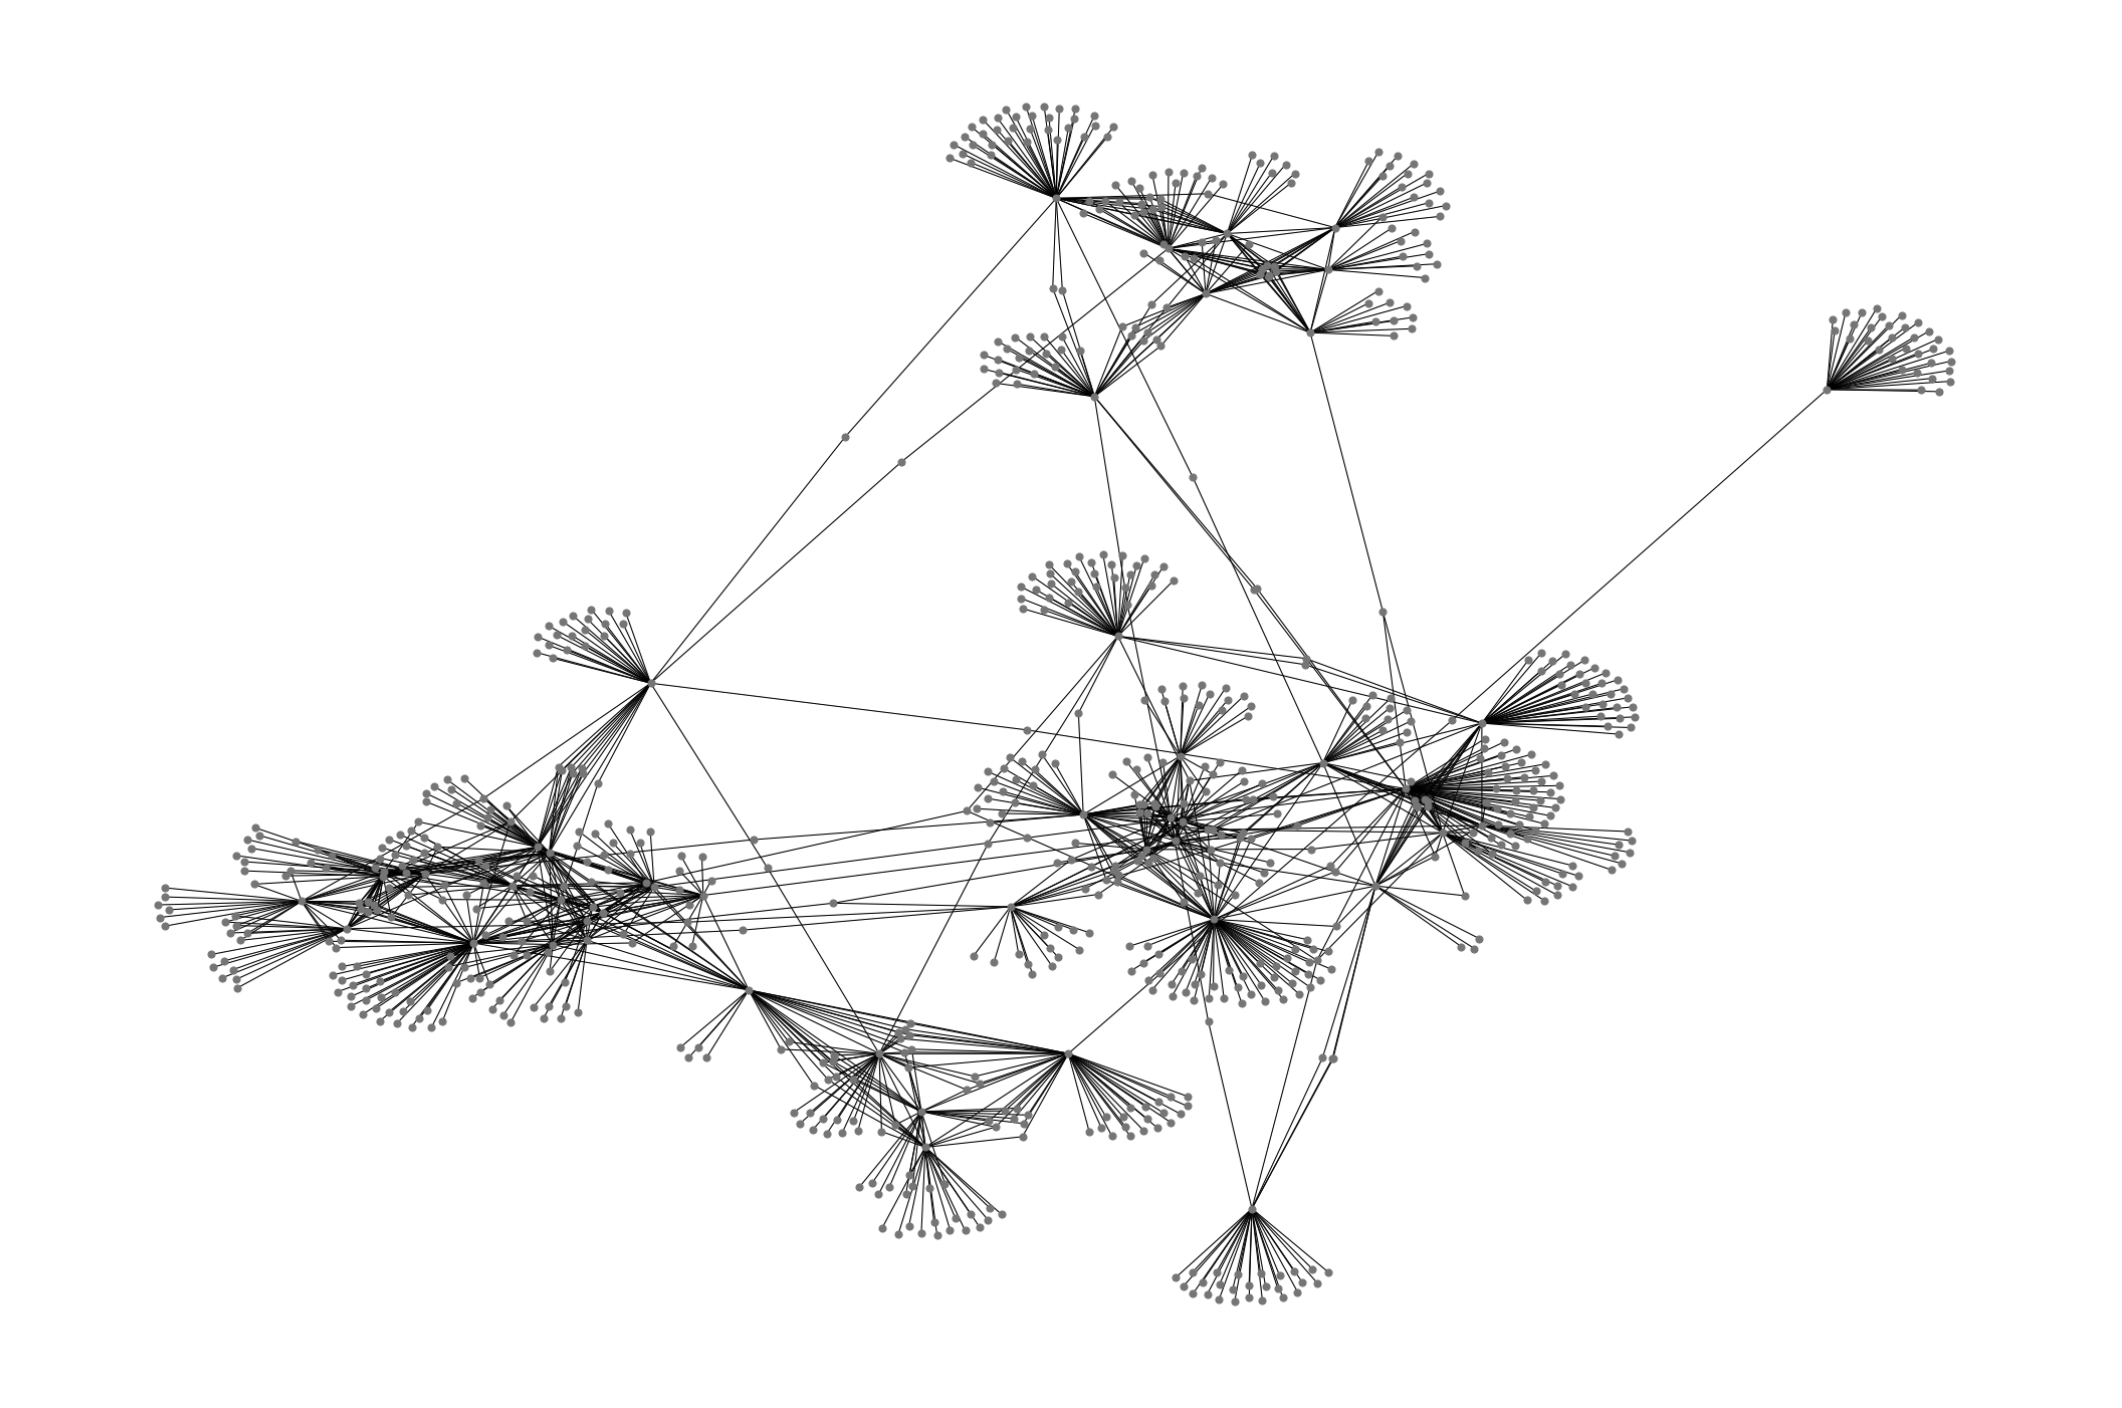
\includegraphics[width=\textwidth]{trr}}
        \caption{TRR network graph}
        \label{trr}
    \end{subfigure}%
    \begin{subfigure}{0.5\textwidth}
        \frame{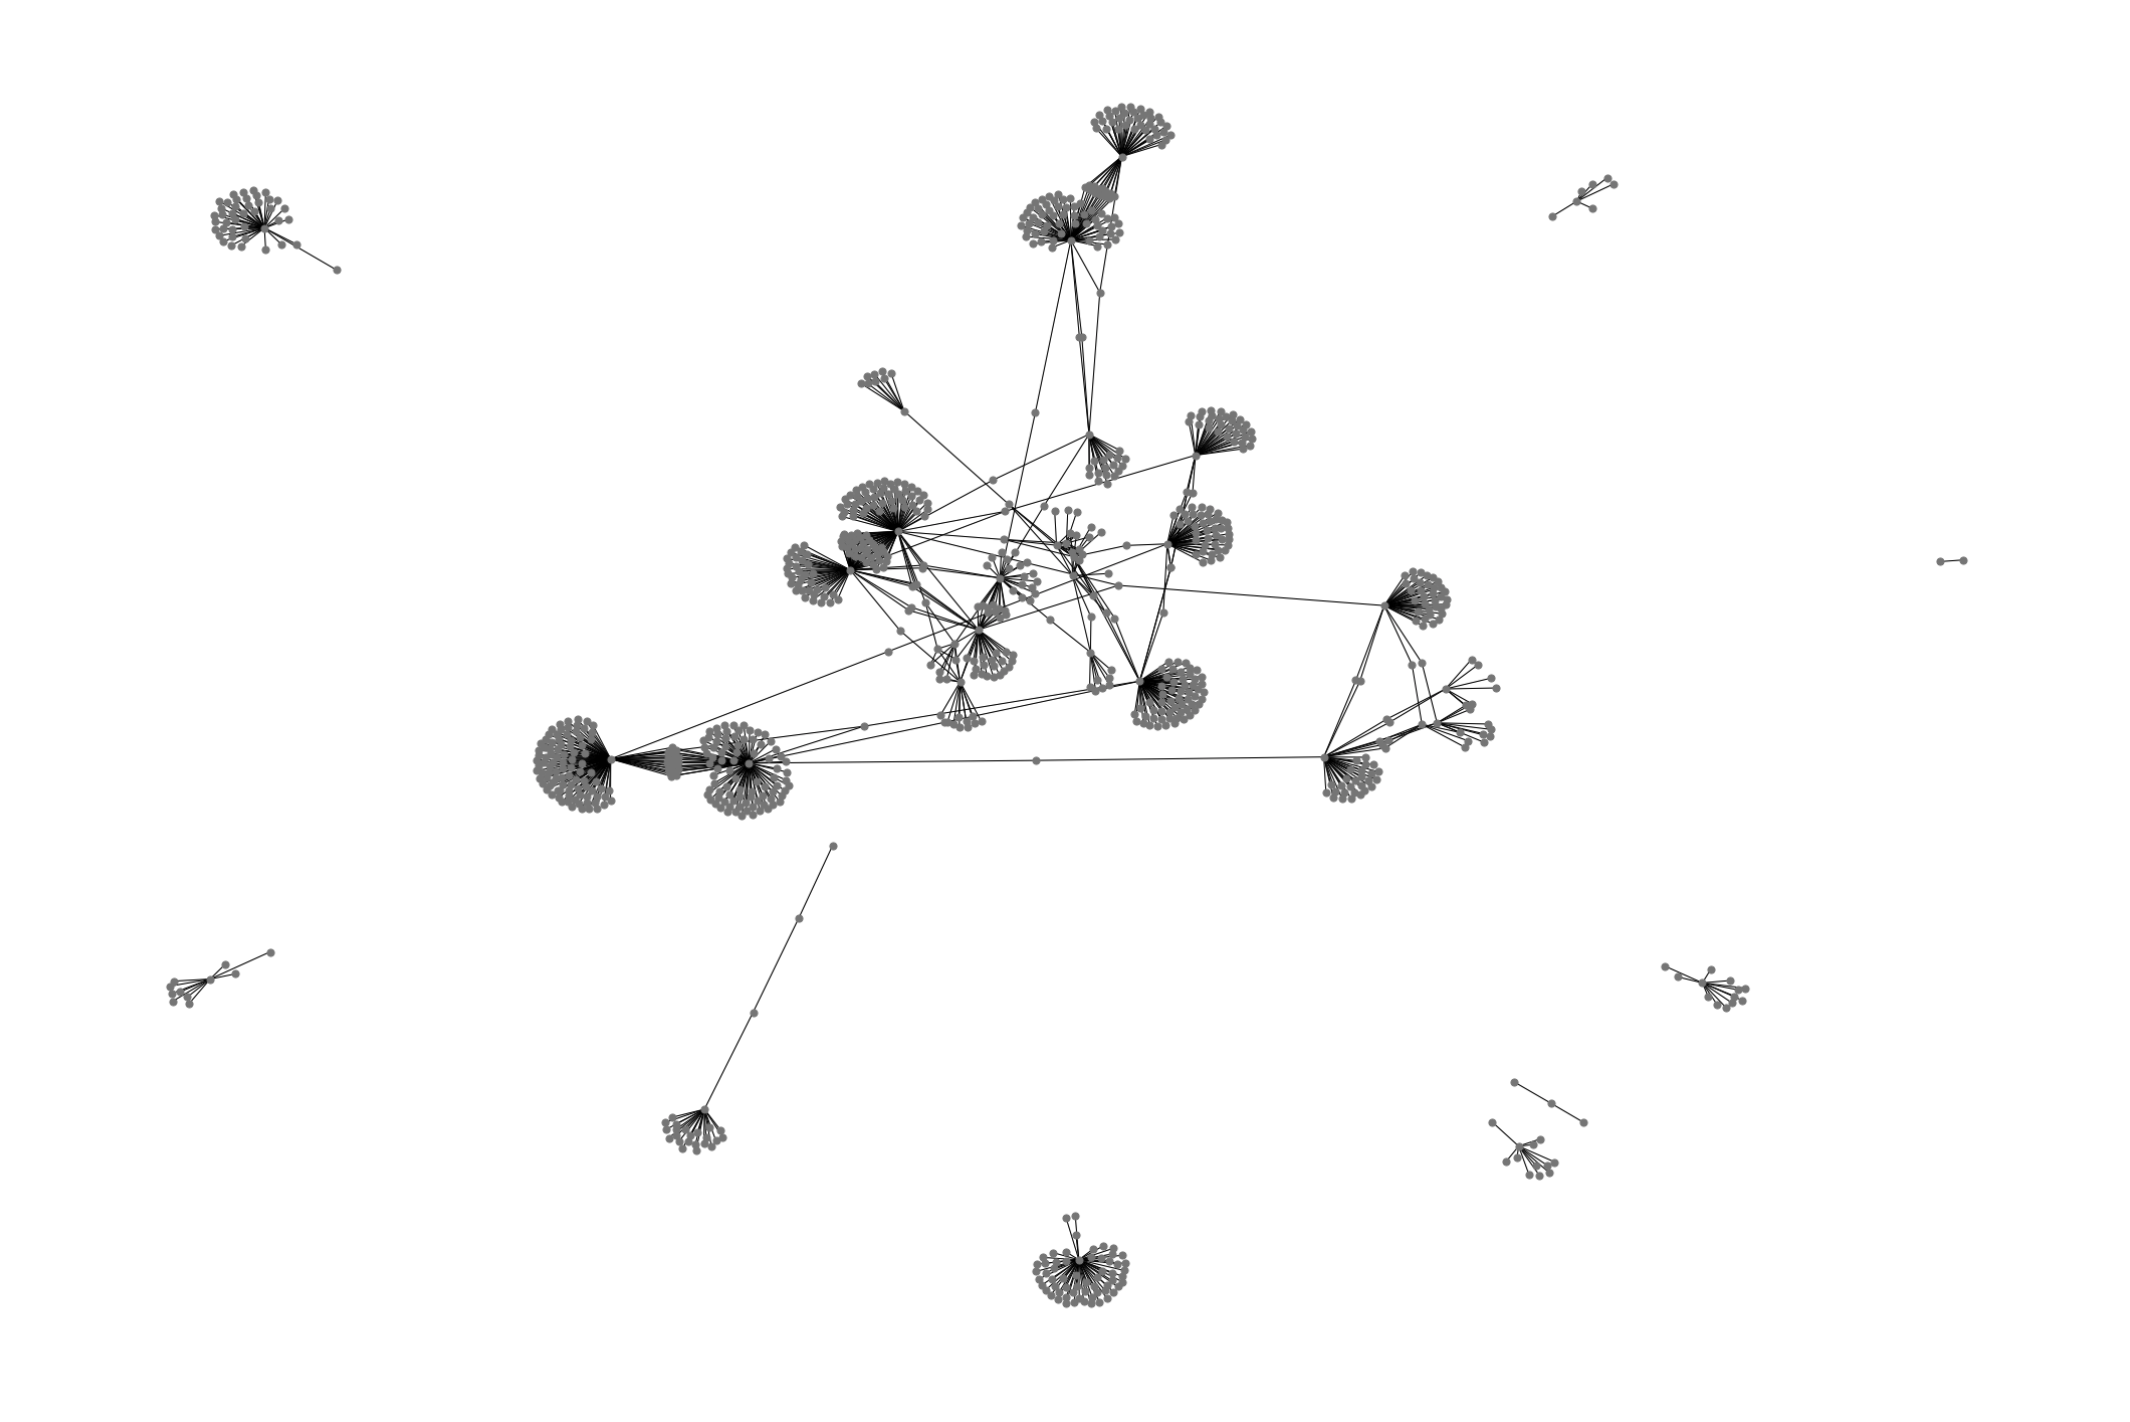
\includegraphics[width=\textwidth]{baseline}}
        \caption{Baseline network graph}
        \label{baseline}
    \end{subfigure}
\caption{TRR network graph and baseline network graph for all TRR cases.}
\end{figure*}

The results in Figure \ref{trr} show that the TRR graph is tightly connected whereas in Figure \ref{baseline} the baseline graph is rather sparse. This indicates that the officers involved in TRR cases are not those who commonly work together.

We also plot the same network graphs for TRR cases involving only cross-race use of force.

\begin{figure*}
\captionsetup{font=small}
    \begin{subfigure}{0.5\textwidth}
        \frame{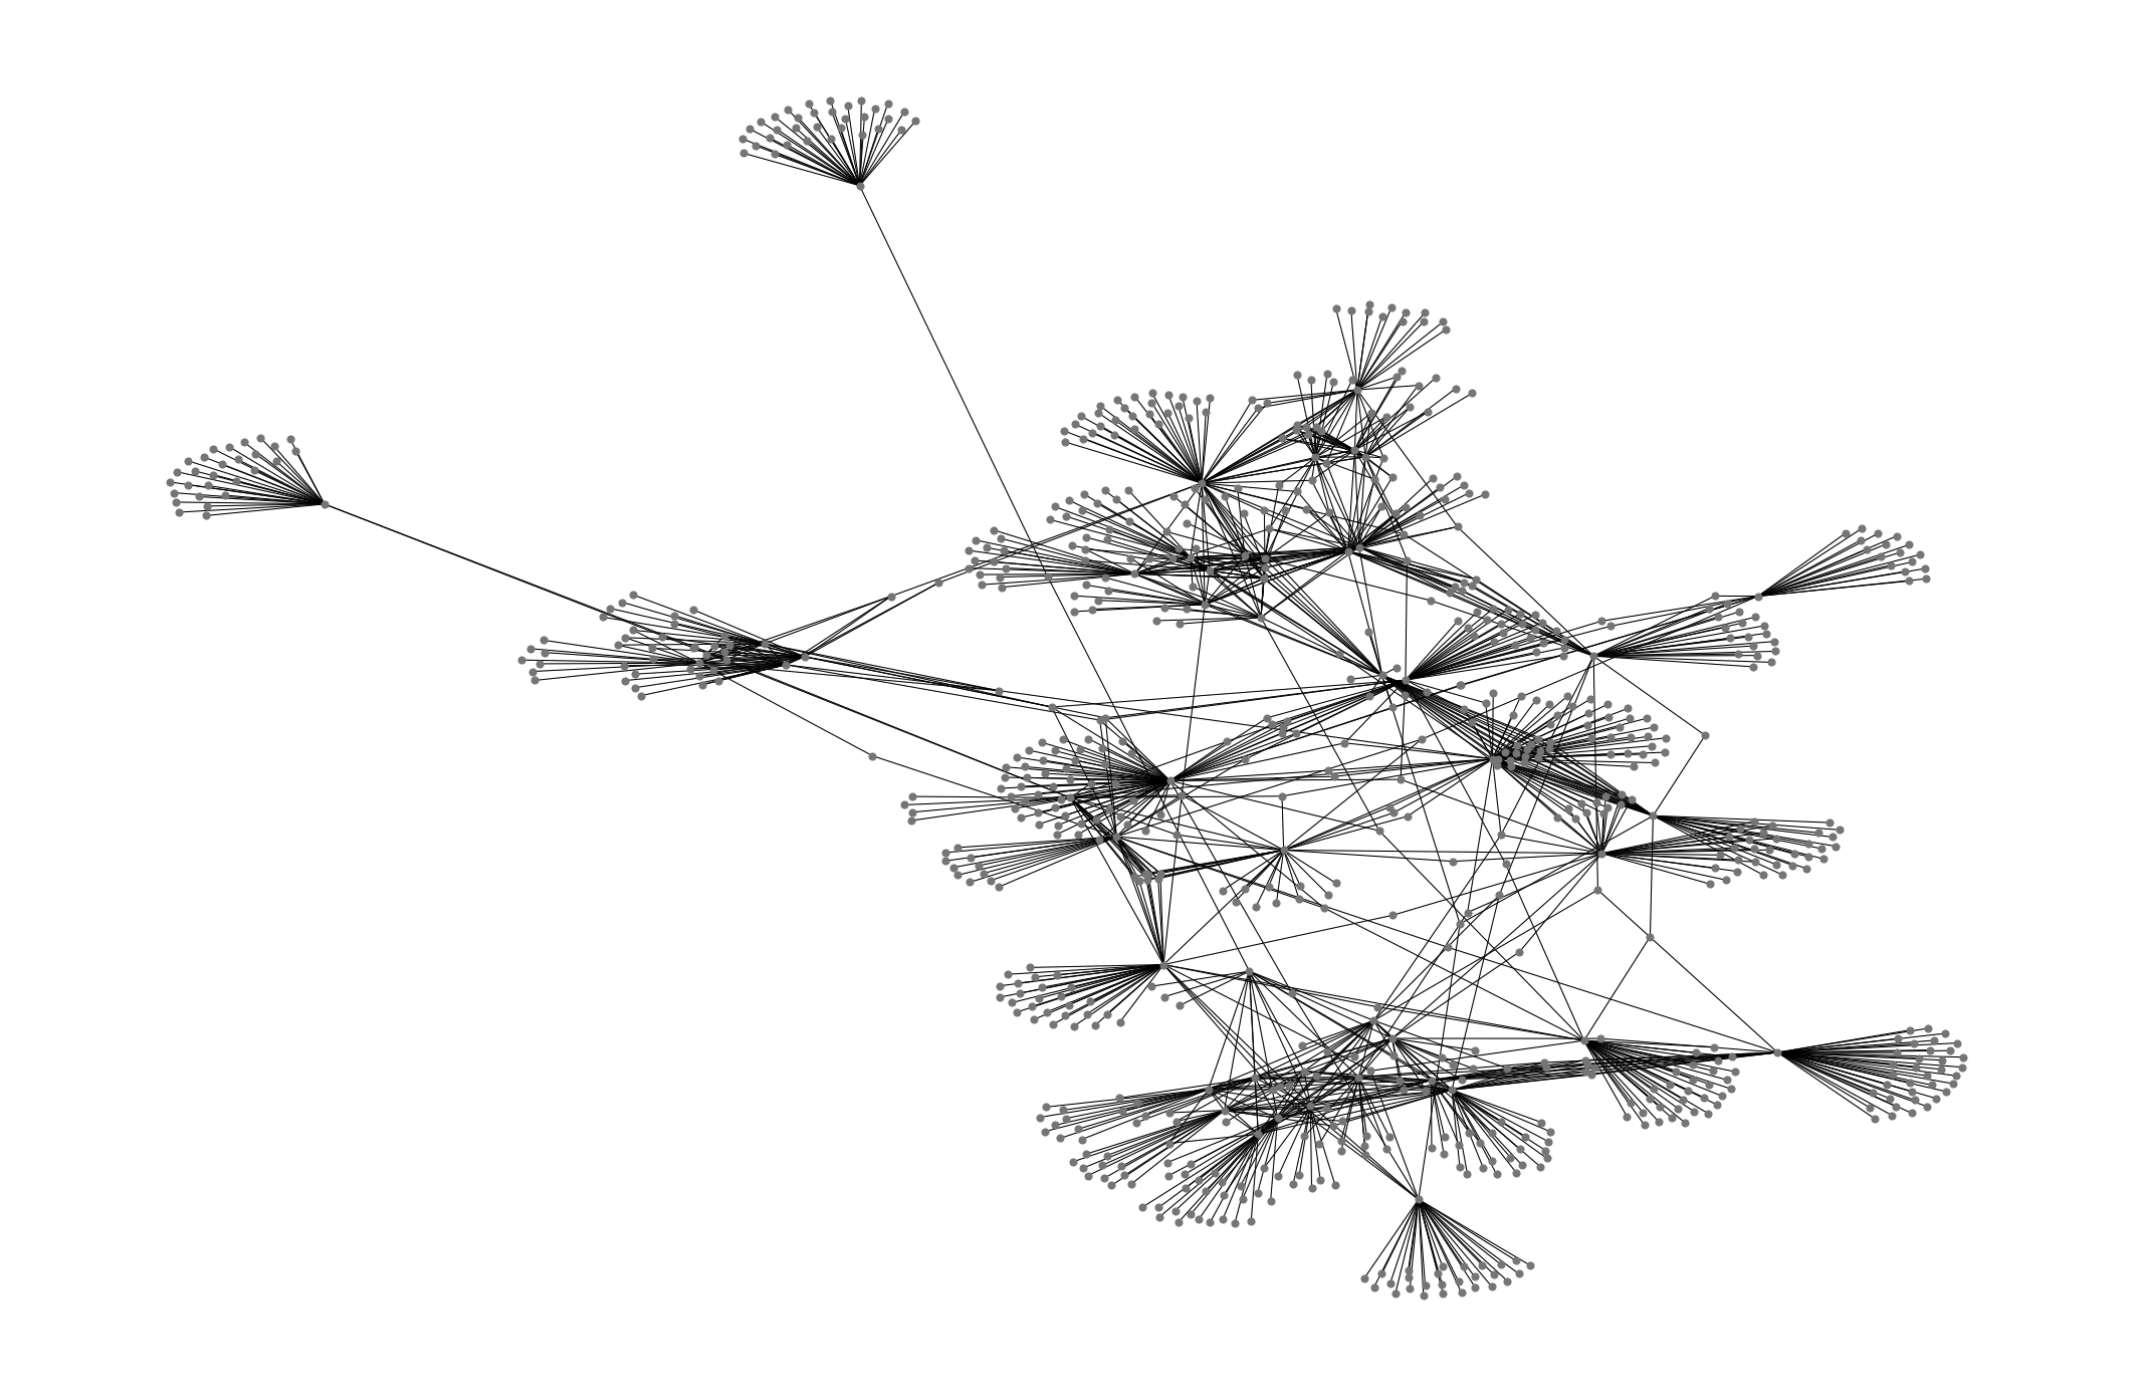
\includegraphics[width=\textwidth]{trr_cross_race}}
        \caption{TRR network graph}
        \label{trr_cross_race}
    \end{subfigure}%
    \begin{subfigure}{0.5\textwidth}
        \frame{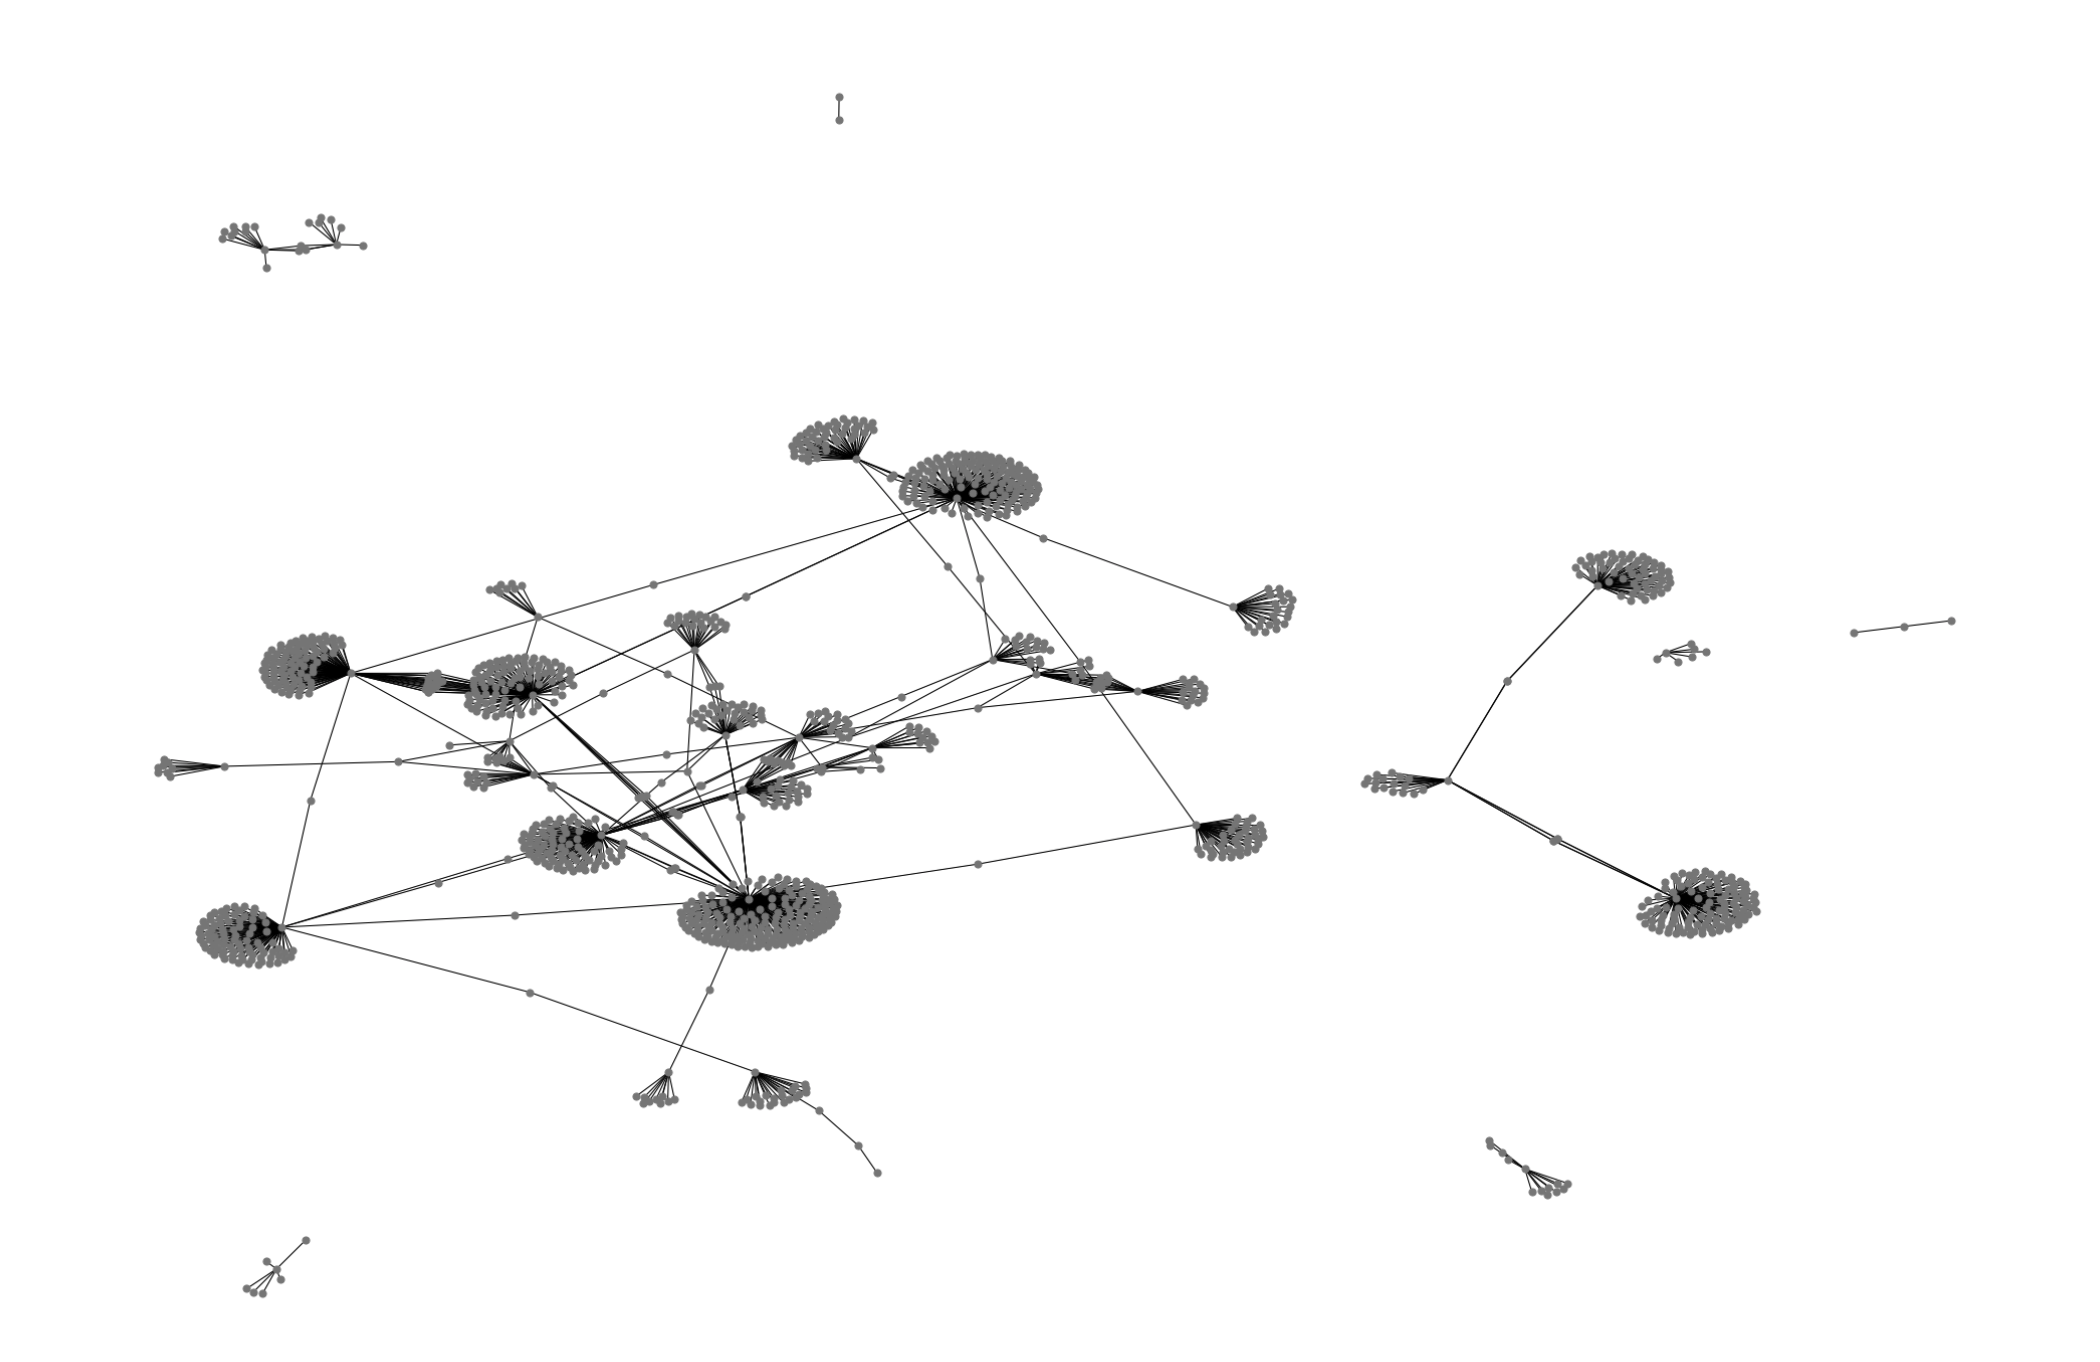
\includegraphics[width=\textwidth]{baseline_cross_race}}
        \caption{Baseline network graph}
        \label{baseline_cross_race}
    \end{subfigure}
\caption{TRR network graph and baseline network graph for TRR cases involving only \textbf{cross-race use of force}.}
\end{figure*}

The graphs in Figure \ref{trr_cross_race} and Figure \ref{baseline_cross_race} show the same results. This indicates that there is a group of offending officers who are responsible for the majority of the TRR cases. Furthermore, they are the one influencing other officers (the ones not commonly engaged in TRR cases). We consider these the ``bad apples".

\begin{figure}[H]
\centering
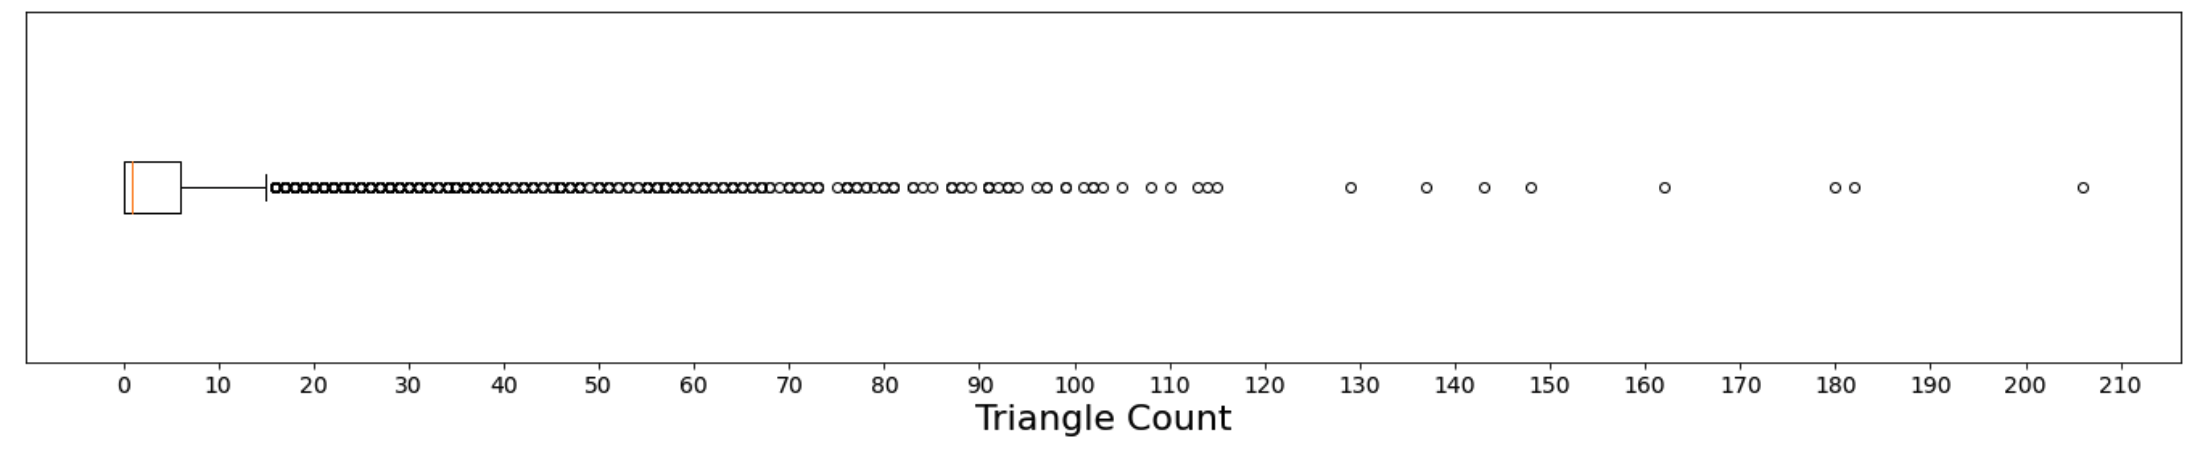
\includegraphics[width=\textwidth]{triangle_count}
\caption{Triangle count boxplot for all TRR cases.}
\label{triangle_count}
\end{figure}

\begin{figure}[H]
\centering
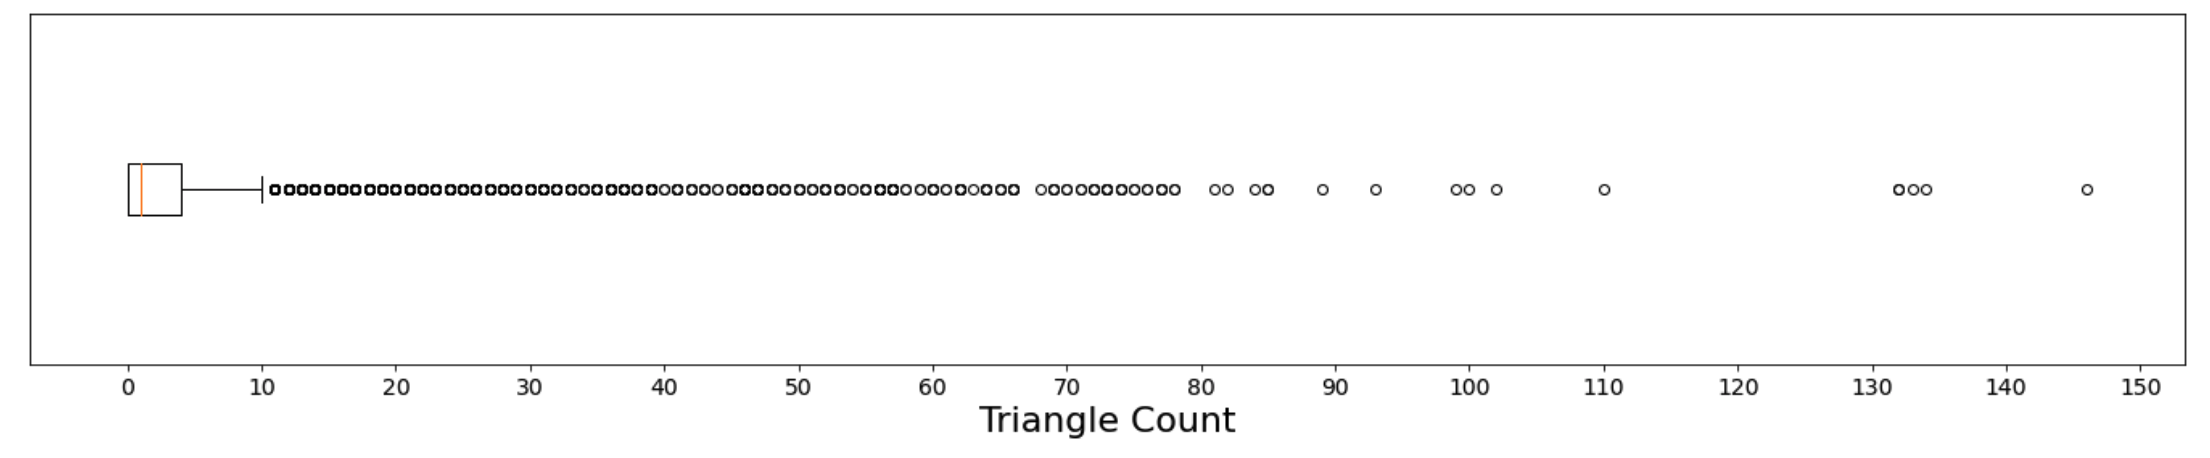
\includegraphics[width=\textwidth]{triangle_count_cross_race}
\caption{Triangle count boxplot for TRR cases involving only \textbf{cross-race use of force}.}
\label{triangle_count_cross_race}
\end{figure}

To further support this hypothesis, we plot boxplots for the triangle counts for TRR cases. Figure \ref{triangle_count} and Figure \ref{triangle_count_cross_race} show that most of the officers with a large number of triangle counts are considered outliers.




\section{Off Shift TRR Analysis}


We hypothesize that officers with relatively more off-shift TRR cases given their total number of TRR cases are surely breaking the rules and actively influencing others with excessive force usage.

To investigate this, we extracted the top 200 ``bad guys" (defined by the officers with the largest difference in their triangle count between TRR event graph and baseline shift graph). Then we extracted the ratio of their number of off-shift TRR over their total number of TRR, as below (``ratio"). Our thought is that officers with the most involvement in TRR community might be the ones who engage in the undesired activities.

We found that, ordering by ``ratio", there are many of them with off-shift TRR. However, the officers with the lowest ratio are those with fewer TRR cases. Most of these officers have a ratio over 0.9, which means off-shift TRR is not quite relevant to active use of force. This disagrees with our original hypothesis. Therefore, a taken-away message could be it’s not going to be very helpful for regulating use of force by monitoring officers' off-shift TRR.




\section{PageRank Analysis}

To further analyze the prominent influencers in this network, we compute the PageRank of each officer in the network graph. Since our edges are originally directed, we need to first convert them to undirected edges by cloning each edge and reversing the source and destination. Then we concatenate the reversed edges with the original edges to produce an undirected graph.

PageRank measures the relative importance of a node within a connected graph. In our case, officers with a higher PageRank value mean they are influencing more officers by being in TRR co-offending cases with more different officers. This measure is similar to the triangle count measure but accounts for influence on a global scale whereas the triangle count is more limited to local influence within tight-knit groups.

\begin{figure}[H]
\centering
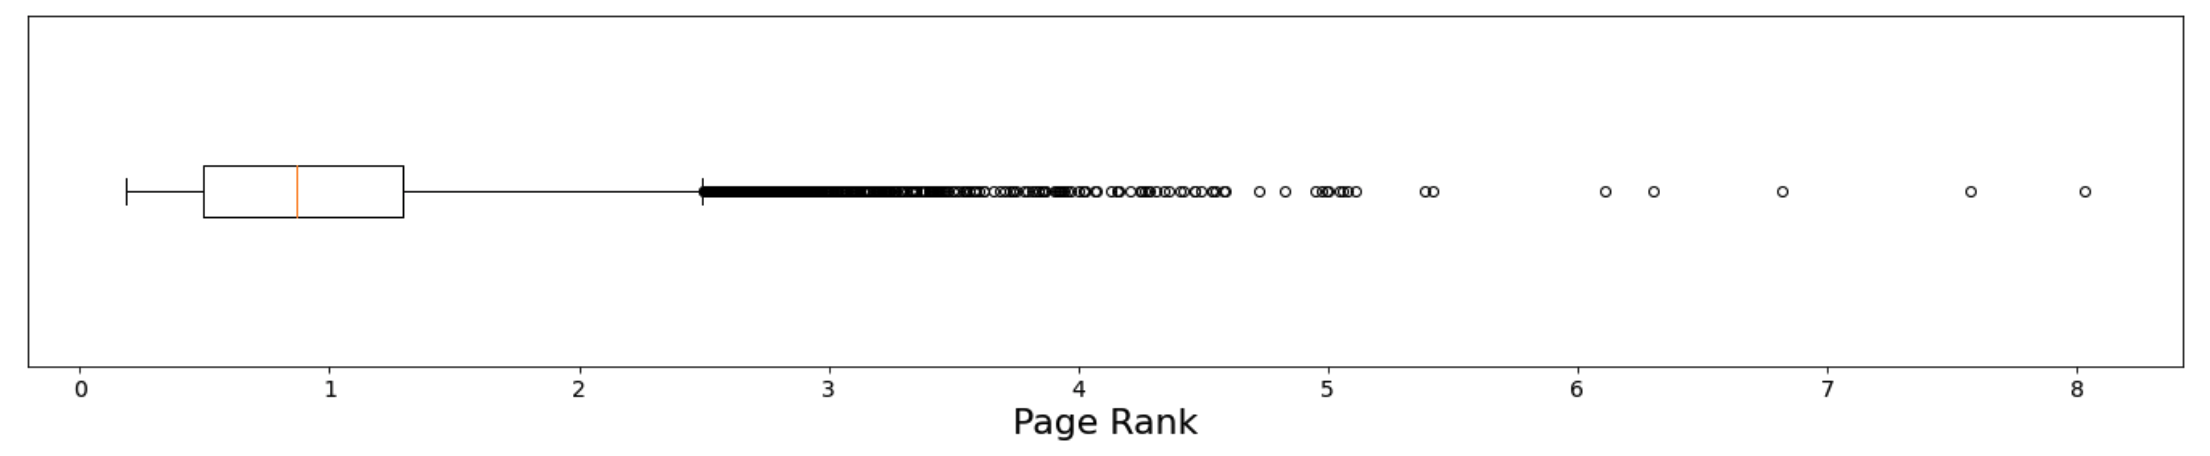
\includegraphics[width=\textwidth]{pr}
\caption{PageRank value boxplot for all TRR cases.}
\label{pr}
\end{figure}

\begin{figure}[H]
\centering
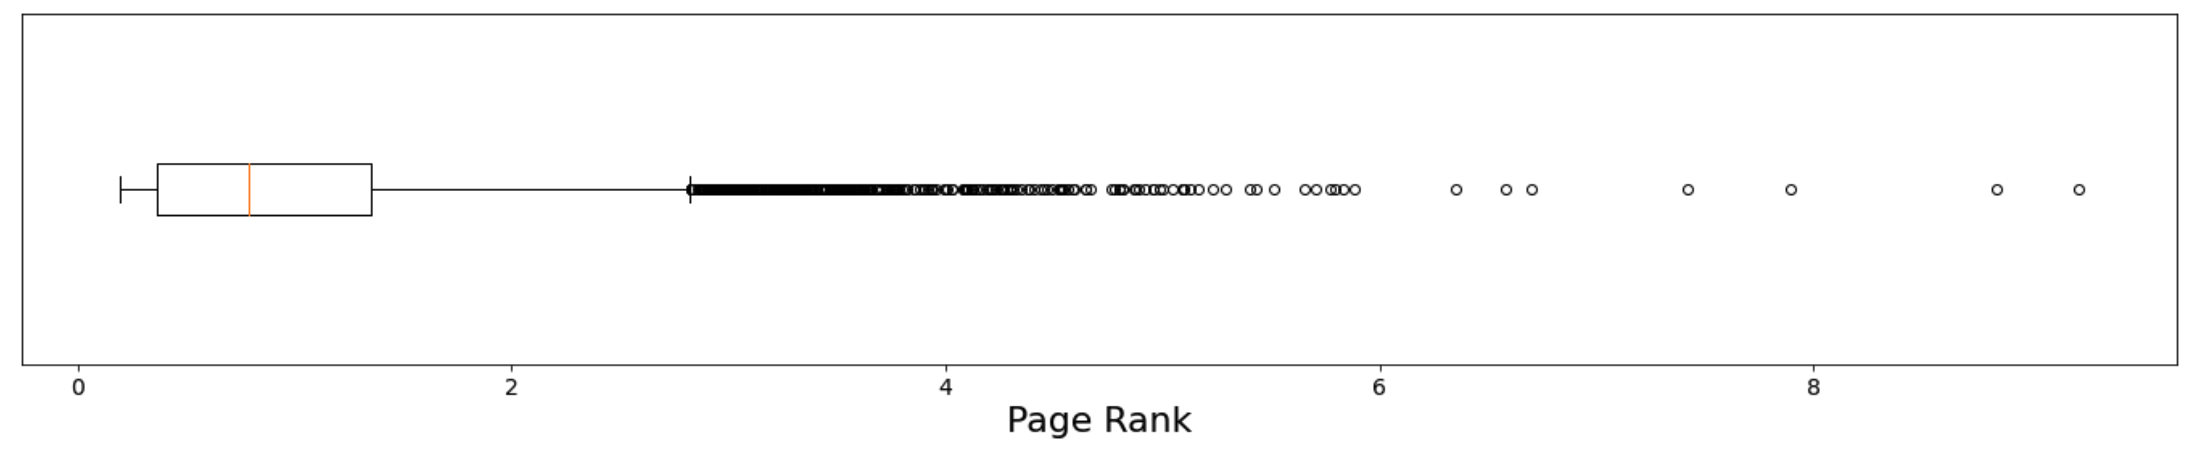
\includegraphics[width=\textwidth]{pr_cross_race}
\caption{PageRank value boxplot for TRR cases involving only \textbf{cross-race use of force}.}
\label{pr_cross_race}
\end{figure}

From Figure \ref{pr} and Figure \ref{pr_cross_race}, we can quickly verify that the most influential officers are outliers in the graph. However, by comparing the 200 most influential officers according to PageRank values, we can see that they are fundamentally different from the influential officers determined by triangle count (100 out of 200 officers are different). This supports our reasoning of the local vs. global influence.


\section{Conclusion and Future Research}

From our graph analysis, we can conclude that there is a group of officers that account for the majority of the TRR cases. These officers are also influencing other officers based on our analysis on co-offending TRR cases. This analysis allows us to dig deeper into the specific, individual cases to discover reasons on why this is the case.

Unfortunately, we didn’t find any evidence of cross-race use of force playing a significant role in this system. For future research, we would look into the individual reports and apply NLP techniques to determine whether racial discrimination plays a role in police use of force.



\end{document}
